\documentclass[14pt]{extbook}
\usepackage{multicol, enumerate, enumitem, hyperref, color, soul, setspace, parskip, fancyhdr} %General Packages
\usepackage{amssymb, amsthm, amsmath, latexsym, units, mathtools} %Math Packages
\everymath{\displaystyle} %All math in Display Style
% Packages with additional options
\usepackage[headsep=0.5cm,headheight=12pt, left=1 in,right= 1 in,top= 1 in,bottom= 1 in]{geometry}
\usepackage[usenames,dvipsnames]{xcolor}
\usepackage{dashrule}  % Package to use the command below to create lines between items
\newcommand{\litem}[1]{\item#1\hspace*{-1cm}\rule{\textwidth}{0.4pt}}
\pagestyle{fancy}
\lhead{Progress Quiz 1}
\chead{}
\rhead{Version C}
\lfoot{5899-4682}
\cfoot{}
\rfoot{Spring 2021}
\begin{document}

\begin{enumerate}
\litem{
Find the equation of the line described below. Write the linear equation as $ y=mx+b $ and choose the intervals that contain $m$ and $b$.\[ \text{Parallel to } 4 x - 5 y = 14 \text{ and passing through the point } (-9, 9). \]\begin{enumerate}[label=\Alph*.]
\item \( m \in [0.49, 1.15] \hspace*{3mm} b \in [17.1, 19.4] \)
\item \( m \in [-0.85, -0.41] \hspace*{3mm} b \in [-0.6, 3.9] \)
\item \( m \in [1.19, 1.26] \hspace*{3mm} b \in [15.1, 17.3] \)
\item \( m \in [0.49, 1.15] \hspace*{3mm} b \in [-18.2, -15.9] \)
\item \( m \in [0.49, 1.15] \hspace*{3mm} b \in [15.1, 17.3] \)

\end{enumerate} }
\litem{
Solve the linear equation below. Then, choose the interval that contains the solution.\[ \frac{9x + 4}{5} - \frac{-4x + 7}{3} = \frac{7x + 6}{4} \]\begin{enumerate}[label=\Alph*.]
\item \( x \in [0.9, 3.3] \)
\item \( x \in [5.1, 7.7] \)
\item \( x \in [-0.6, 1.7] \)
\item \( x \in [-2.3, 0.2] \)
\item \( \text{There are no real solutions.} \)

\end{enumerate} }
\litem{
Solve the equation below. Then, choose the interval that contains the solution.\[ -3(12x + 17) = -9(2x -14) \]\begin{enumerate}[label=\Alph*.]
\item \( x \in [3.17, 6.17] \)
\item \( x \in [-4.17, -0.17] \)
\item \( x \in [-11.83, -5.83] \)
\item \( x \in [0.39, 3.39] \)
\item \( \text{There are no real solutions.} \)

\end{enumerate} }
\litem{
First, find the equation of the line containing the two points below. Then, write the equation as $ y=mx+b $ and choose the intervals that contain $m$ and $b$.\[ (-2, -6) \text{ and } (-5, 7) \]\begin{enumerate}[label=\Alph*.]
\item \( m \in [-6.33, -3.33] \hspace*{3mm} b \in [6, 14] \)
\item \( m \in [-6.33, -3.33] \hspace*{3mm} b \in [-18.67, -7.67] \)
\item \( m \in [2.33, 8.33] \hspace*{3mm} b \in [26.67, 31.67] \)
\item \( m \in [-6.33, -3.33] \hspace*{3mm} b \in [-9, -3] \)
\item \( m \in [-6.33, -3.33] \hspace*{3mm} b \in [12.67, 17.67] \)

\end{enumerate} }
\litem{
First, find the equation of the line containing the two points below. Then, write the equation as $ y=mx+b $ and choose the intervals that contain $m$ and $b$.\[ (-7, 10) \text{ and } (5, 8) \]\begin{enumerate}[label=\Alph*.]
\item \( m \in [-0.7, -0.1] \hspace*{3mm} b \in [2.8, 5.1] \)
\item \( m \in [-0.7, -0.1] \hspace*{3mm} b \in [16.6, 17.4] \)
\item \( m \in [0, 1] \hspace*{3mm} b \in [4.4, 8.7] \)
\item \( m \in [-0.7, -0.1] \hspace*{3mm} b \in [7.9, 14.3] \)
\item \( m \in [-0.7, -0.1] \hspace*{3mm} b \in [-10.5, -8.4] \)

\end{enumerate} }
\litem{
Write the equation of the line in the graph below in Standard form $Ax+By=C$. Then, choose the intervals that contain $A, B, \text{ and } C$.
\begin{center}
    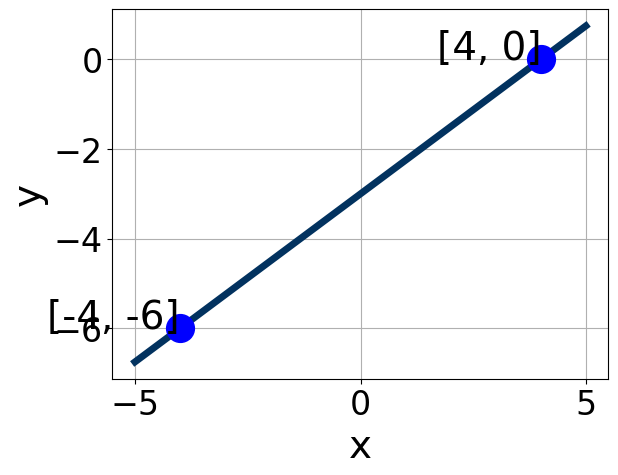
\includegraphics[width=0.5\textwidth]{../Figures/linearGraphToStandardCopyC.png}
\end{center}
\begin{enumerate}[label=\Alph*.]
\item \( A \in [4, 7], \hspace{3mm} B \in [3.7, 4.3], \text{ and } \hspace{3mm} C \in [-16, -10] \)
\item \( A \in [-6, -2], \hspace{3mm} B \in [-4.87, -3.18], \text{ and } \hspace{3mm} C \in [16, 19] \)
\item \( A \in [-1.75, 2.25], \hspace{3mm} B \in [0.57, 1.06], \text{ and } \hspace{3mm} C \in [-4, 1] \)
\item \( A \in [-1.75, 2.25], \hspace{3mm} B \in [-2.05, -0.22], \text{ and } \hspace{3mm} C \in [4, 9] \)
\item \( A \in [4, 7], \hspace{3mm} B \in [-4.87, -3.18], \text{ and } \hspace{3mm} C \in [16, 19] \)

\end{enumerate} }
\litem{
Write the equation of the line in the graph below in Standard form $Ax+By=C$. Then, choose the intervals that contain $A, B, \text{ and } C$.
\begin{center}
    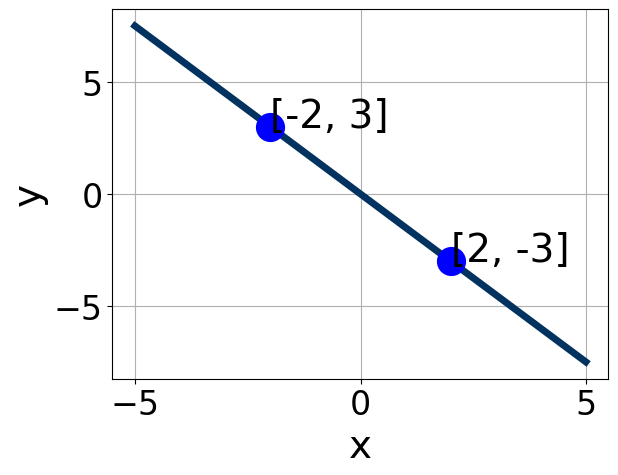
\includegraphics[width=0.5\textwidth]{../Figures/linearGraphToStandardC.png}
\end{center}
\begin{enumerate}[label=\Alph*.]
\item \( A \in [-1.67, 1.33], \hspace{3mm} B \in [-0.53, 1.17], \text{ and } \hspace{3mm} C \in [-5, 1] \)
\item \( A \in [1, 10], \hspace{3mm} B \in [2.19, 4.71], \text{ and } \hspace{3mm} C \in [-15, -5] \)
\item \( A \in [1, 10], \hspace{3mm} B \in [-3.69, -2.09], \text{ and } \hspace{3mm} C \in [8, 11] \)
\item \( A \in [-6, -3], \hspace{3mm} B \in [2.19, 4.71], \text{ and } \hspace{3mm} C \in [-15, -5] \)
\item \( A \in [-1.67, 1.33], \hspace{3mm} B \in [-1.73, 0.96], \text{ and } \hspace{3mm} C \in [3, 8] \)

\end{enumerate} }
\litem{
Solve the equation below. Then, choose the interval that contains the solution.\[ -19(4x -18) = -16(17x + 15) \]\begin{enumerate}[label=\Alph*.]
\item \( x \in [-0.77, -0.5] \)
\item \( x \in [0.43, 0.67] \)
\item \( x \in [-0.07, 0.42] \)
\item \( x \in [-3.25, -2.69] \)
\item \( \text{There are no real solutions.} \)

\end{enumerate} }
\litem{
Find the equation of the line described below. Write the linear equation as $ y=mx+b $ and choose the intervals that contain $m$ and $b$.\[ \text{Perpendicular to } 8 x + 5 y = 12 \text{ and passing through the point } (8, -4). \]\begin{enumerate}[label=\Alph*.]
\item \( m \in [-1, -0.03] \hspace*{3mm} b \in [0, 4] \)
\item \( m \in [0.58, 0.86] \hspace*{3mm} b \in [8, 10] \)
\item \( m \in [0.96, 1.88] \hspace*{3mm} b \in [-9, -6] \)
\item \( m \in [0.58, 0.86] \hspace*{3mm} b \in [-12, -10] \)
\item \( m \in [0.58, 0.86] \hspace*{3mm} b \in [-9, -6] \)

\end{enumerate} }
\litem{
Solve the linear equation below. Then, choose the interval that contains the solution.\[ \frac{-6x -7}{8} - \frac{-3x + 7}{2} = \frac{4x + 5}{4} \]\begin{enumerate}[label=\Alph*.]
\item \( x \in [5.5, 8.5] \)
\item \( x \in [-1.8, 0.2] \)
\item \( x \in [-23.5, -21.5] \)
\item \( x \in [-76, -75] \)
\item \( \text{There are no real solutions.} \)

\end{enumerate} }
\end{enumerate}

\end{document}